\documentclass[notes=hide,yellow]{beamer}

% (c) 2008 Steffen Klemer <moh AT gmx BEEP org>
% This work is licensed under the Creative Commons Attribution-Share Alike 3.0
% Germany License. To view a copy of this license, visit
% http://creativecommons.org/licenses/by-sa/3.0/de/ or send a letter to Creative
% Commons, 171 Second Street, Suite 300, San Francisco, California, 94105, USA.
%
% See http://www.noch-mehr-davon.de/vortr.shtml
% Permissions beyond the scope of this license may be available at the same site
%
% Template based on: Copyright 2004 by Till Tantau <tantau@users.sourceforge.net>.


\mode<presentation>
{
%	\usetheme{AnnArbor} %Szeged
%	\usetheme{Berkeley}
	\usetheme{Dresden}
%	\usecolortheme{rose} %oder beaver oder rose oder orchid, albatross, rose
% 	\useinnertheme{circles}
%	\useoutertheme{split}
%	\setbeamercovered{invisible} %or transparent
% 	\usefottheme{professionalfonts}
% 	\usefonttheme[onlymath]{serif}
        %\setbeamercovered{invisible}
%	\setbeamertemplate{navigation symbols}{}
}

\usepackage{amsmath,amssymb,latexsym}
\usepackage{fancyvrb}
\usepackage{graphicx}
\usepackage{epstopdf}
\usepackage{amsfonts}
\usepackage{amsthm}
\usepackage{wasysym}
\usepackage{ucs}
\usepackage{stmaryrd}
\usepackage{hyperref}
\usepackage{graphics}
\usepackage{colortbl}
\usepackage[ngerman]{babel}
\usepackage[utf8x]{inputenc}
\usepackage{tikz}
%\usepackage[sort&compress]{natbib}
\usepackage{listings}



 
\lstset{ %
  basicstyle=\tiny,           % the size of the fonts that are used for the code
  numbers=left,                   % where to put the line-numbers
  numberstyle=\tiny\color{gray},  % the style that is used for the line-numbers
  stepnumber=1,                   % the step between two line-numbers. If it's 1, each line 
                                  % will be numbered
  numbersep=5pt,                  % how far the line-numbers are from the code
  backgroundcolor=\color{white},      % choose the background color. You must add \usepackage{color}
  showspaces=false,               % show spaces adding particular underscores
  showstringspaces=false,         % underline spaces within strings
  showtabs=false,                 % show tabs within strings adding particular underscores
  frame=single,                   % adds a frame around the code
  rulecolor=\color{black},        % if not set, the frame-color may be changed on line-breaks within not-black text (e.g. commens (green here))
  tabsize=2,                      % sets default tabsize to 2 spaces
  captionpos=b,                   % sets the caption-position to bottom
  breaklines=true,                % sets automatic line breaking
  breakatwhitespace=false,        % sets if automatic breaks should only happen at whitespace
  title=\lstname,                   % show the filename of files included with \lstinputlisting;
                                  % also try caption instead of title
  keywordstyle=\color{blue},          % keyword style
  commentstyle=\color{dkgreen},       % comment style
  stringstyle=\color{mauve},         % string literal style
  escapeinside={\%*}{*)},            % if you want to add LaTeX within your code
  morekeywords={*,...}               % if you want to add more keywords to the set
}

\title{Das verteilte Filesystem Ceph als Storage-Lösung}
\subtitle{ }
\author{Ralph Krimmel}



\begin{document}
	\nocite{*} 
	\begin{frame}
		\titlepage
	\end{frame}

	\begin{frame}
		\tableofcontents
	\end{frame}


\section{Einf\"uhrung}
\subsection*{}

\begin{frame}{Motivation}

\begin{itemize}
	\item Institut f\"ur Numerische und Angwandte Mathematik
	\item \textasciitilde 50 Mitarbeiter
	\item Hardware: 10 inhomogene Server
	\item Kein SAN
	\item Dienste (schon teilweise virtualisiert)
	\begin{itemize}
		\item Fileserver
		\item Webserver
		\item Email \& Groupware
		\item Jabber
		\item Diverse Lizenzserver
		\item Versionsverwaltung (svn, git, hg)
		\item ...
	\end{itemize}
\end{itemize}
\end{frame}

\begin{frame}{Probleme}

	\begin{itemize}
		\item Fileserver
			\begin{itemize}
				\item Dateisystem: ZFS 
				\item Netzwerkdateisystem: NFS
				\item \glqq Hot spare Replikation\grqq 
				\item $\Rightarrow$ Nadel\"ohr
			\end{itemize} 
		\item <2> Restliche Server
			\begin{itemize}
				\item Unbenutzte Speicherkapazit\"at
				\item Unbenutzte Rechenapazit\"at
				\item Unzureichende Verf\"ugbarkeit bei Fehlern
			\end{itemize}
	\end{itemize}
\end{frame}

\begin{frame}{Fileserver Availability}
	\begin{center}
	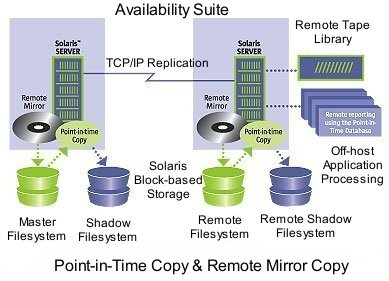
\includegraphics[width=0.65\textwidth]{availabilitysuitenew.jpg}
	\end{center}
	\small
	Quelle: \texttt{http://hub.opensolaris.org/bin/view/Project+avs/}
\end{frame}


\begin{frame}{L\"osungsansatz}
	
	\begin{itemize}
		\item Jeder Server wird Hypervisor
		\item Verteiltes Dateisystem 
	%		\begin{itemize}
	%			\item Ausfalltoleranz (Verf\"ugbarkeit und Zuverl\"assigkeit) durch Replikation
	%			\item Hohe Performanz durch Striping %Aufteilen der Daten auf mehrere physikalische Devices
	%		\end{itemize}
		\item <2> \glqq Private Cloud\grqq ;)
	\end{itemize}

\end{frame}

\begin{frame}{Definition}
		In computing, a distributed file system or network file system is any file system that allows access to files from multiple hosts via a computer network.$[1]$
	\tiny{$[1]$ Galvin Silberschatz (1994). Operating System concepts, chapter 17 Distributed file systems. Addison-Wesley Publishing Company.} \\ 
\end{frame}

\begin{frame}{Nichts neues...}

		z.B. NFS, entwickelt von Sun Microsystems in 1984
		\begin{center}
			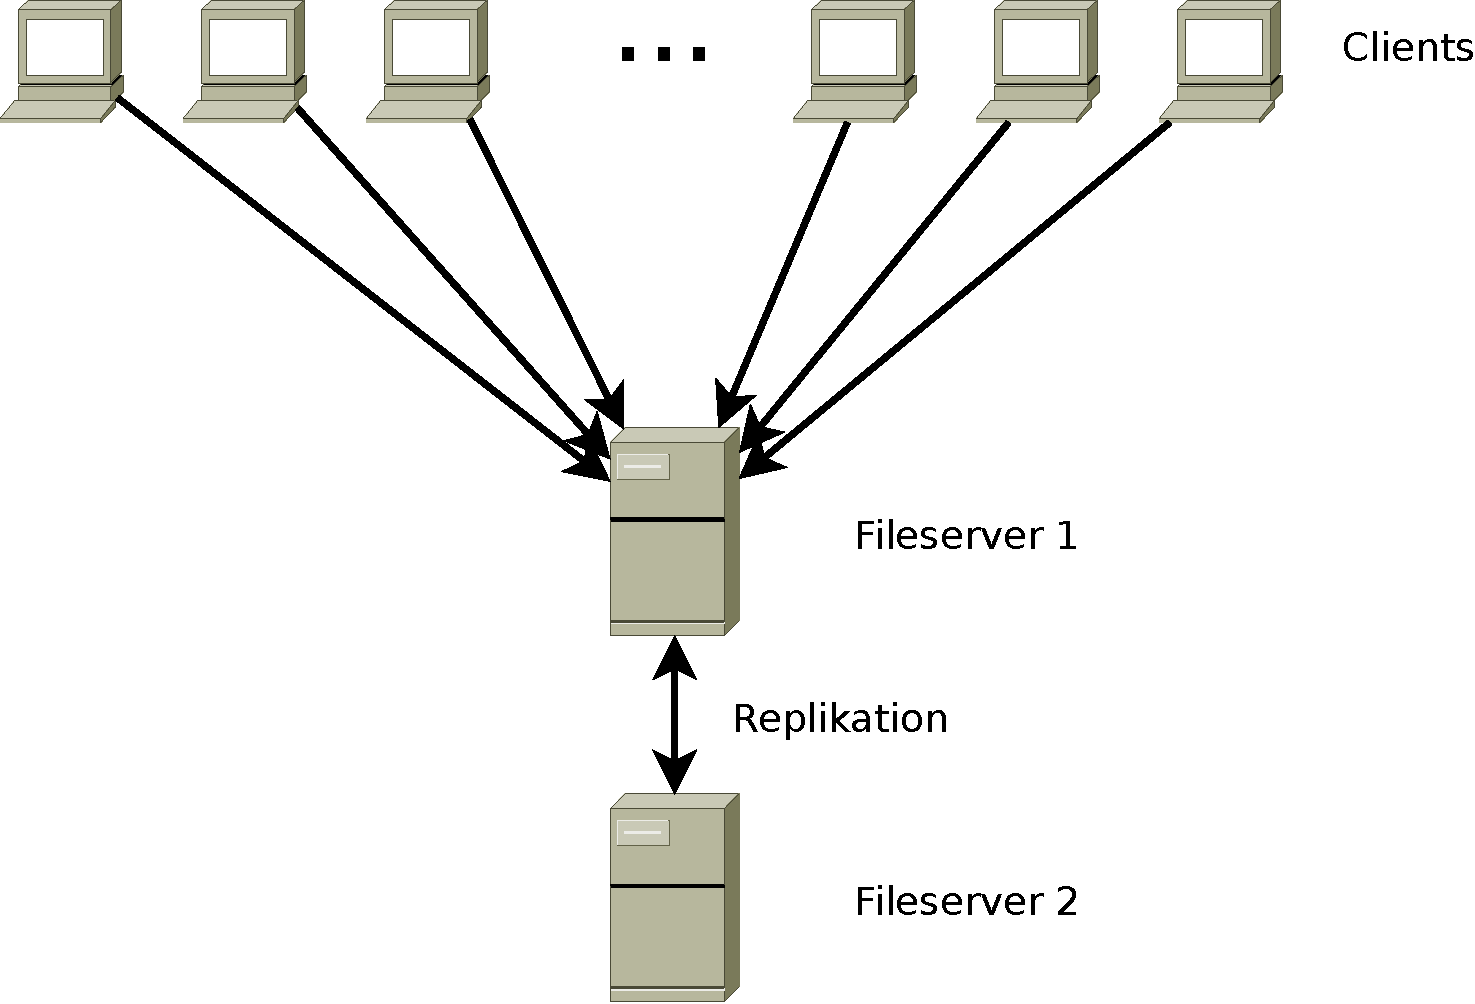
\includegraphics[scale=0.2]{nfs.pdf}
		\end{center}
		\begin{itemize}
			\item Schlechte Performanz bei vielen Clients \\ $\Rightarrow$ Skaliert nicht
			\item Keine Fehlertoleranz
		\end{itemize}
\end{frame}



\begin{frame}{Anforderungen an ein modernes, verteiltes Dateisystem}
	\begin{itemize}
		\item Hohe Performanz durch Striping
			\begin{itemize}
				\item Durchsatz
				\item Latenz
			\end{itemize}
		\item Skalierbarkeit
		\item Verf\"ugbarkeit
		\item Zuverl\"assigkeit
	\end{itemize}
\end{frame}

\begin{frame}{Zuverl\"assigkeit/Verf\"ugbarkeit}
	Problem: Fehler sind mehr die Norm als die Ausnahme
	\begin{itemize}
		\item System g\"unstiger Hardware
		\item Fehler in Programmen %theres software that always crashes 
		\item Menschliches Versagen % what was this cable for?
		\item Betriebssystemfehler % ever used windows?
		\item Ausfall von: 
		\begin{itemize}
			\item Festplatten
			\item Arbeitsspeicher
			\item Kabel
			\item Netzwerk
			\item ...
		\end{itemize}
	\end{itemize}		
\end{frame}

\begin{frame}{Moderner Ansatz}
	\begin{itemize}
		\item Objektbasiert
		\item Festplatten $\rightarrow$ Intelligent object storage devices (OSD's)
		\begin{itemize}
			\item CPU
			\item Netzwerkschnittstelle
			\item Lokaler Cache
		\end{itemize}
		\item Metadaten getrennt von Nutzdaten
	\end{itemize}
\end{frame}


\begin{frame}{Typischer Zugriff (z.B. Hadoop)}
	\begin{center}
	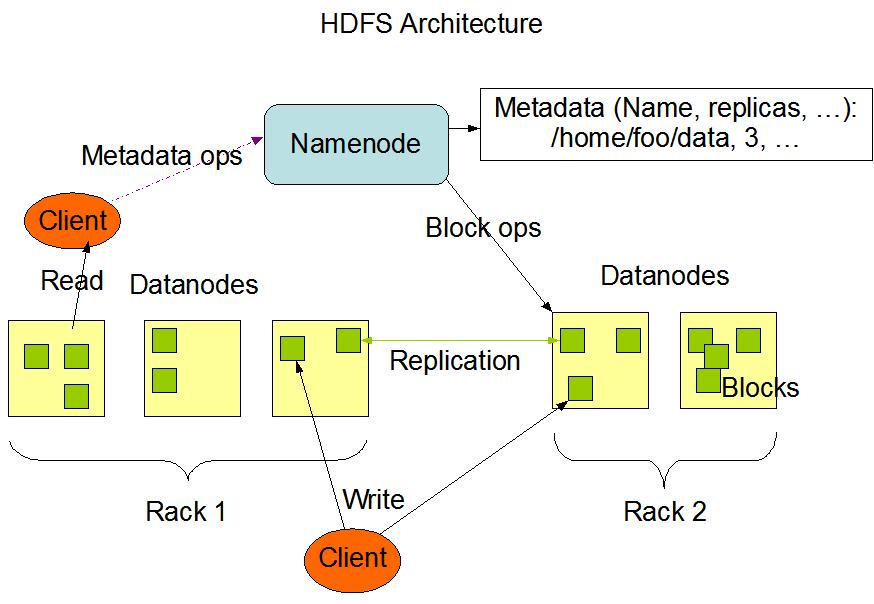
\includegraphics[scale=0.2]{hdfsarchitecture.jpg}
	\end{center}
	\small
	Quelle: \texttt{http://hadoop.apache.org/common/docs/r0.20.2/hdfs\_design.html}
\end{frame}


\begin{frame}{Weitere verteilte Dateisysteme}
	\begin{center}
		\begin{tabular}{|c|c|}
		\hline
		Dateisystem & Bemerkung \\
		\hline
		Lustre & Alter Kernel \\
		Google File System & Propriet\"ar, ausgelegt auf große Dateien \\
		GlusterFS & Nur FUSE, Alternative? Meinungen?\\
		\hline
	\end{tabular}
	\end{center}
\end{frame}


\section{Ceph - Theorie}
\subsection*{}

\begin{frame}
	\begin{center}
	\Large{Ceph}
	\end{center}
\end{frame}

\begin{frame}{Ceph - \"Ubersicht}
	
	Drei Komponenten:
	\begin{itemize}
		\item Client: Posix\"ahnliche Schnittstelle %Stellt zur verfuegung
		\item OSD Cluster: Speichert Daten und Metadaten
		\item Metadaten Cluster
			\begin{itemize}
				\item Verwaltet Namensraum
				\item Konsistenz/Koh\"arenz
				\item Sicherheit (Noch nicht ausreichend implementiert)
			\end{itemize}
	\end{itemize}
\end{frame}

\begin{frame}
	\begin{center}
		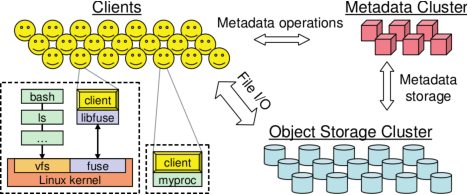
\includegraphics{ceph_architecture.pdf}
	\end{center}
	Quelle: \cite{weil2006}
\end{frame}


\begin{frame}{Design Features}
	\begin{itemize}
		\item Trennung der Verwaltung von Daten und Metadaten
		\begin{itemize}
			\item Unabhaengige Skalierbarkeit
			\item Keine Block/Objektlisten (CRUSH)
		\end{itemize}
		\item  Dynamische Verteilung der Metadaten
		\begin{itemize}
			\item Halber Aufwand sind Metadatenoperationen
			\item Gutes Loadbalancing der Metadaten ist \"außerst wichtig %fuer performance
		\end{itemize}
		\item Autonomes OSD Cluster verantwortlich f\"ur:
			\begin{itemize}
				\item Replikation
				\item Fehlererkennung
				\item Wiederherstellung nach Fehlern
			\end{itemize}
	\end{itemize}	
\end{frame}

\begin{frame}{Dateizugriff}

\begin{enumerate}
	\item Client sendet Dateirequest an das MDS Cluster
	\item Ein MDS \"ubersetzt Dateiname in \textit{file inode}
	\begin{itemize}
		\item Unique inode number
		\item Besitzer
		\item Gr\"oße
		\item ...
	\end{itemize}
	\item MDS gibt inode number, Gr\"oße und Verteilungsstrategie zur\"uck
	\item Direkter Zugriff von Client auf OSD
\end{enumerate}
\end{frame}

\begin{frame}{Client Synchronisierung}
	Problem: Mehrere Clients schreiben lesen eine Datei gleichzeitig.

	\begin{itemize}	
		\item Kein read caching/write buffering mehr
		\item I/O der clients synchron %blocked until acked
			\begin{itemize}
				\item Synchrone I/O schlecht f\"ur Client Performanz
			\end{itemize}
		\item HPC Erweiterung: O\_LAZY flag f\"ur \texttt{open}
	\end{itemize}
\end{frame}


\begin{frame}{CRUSH}
	\begin{center}
	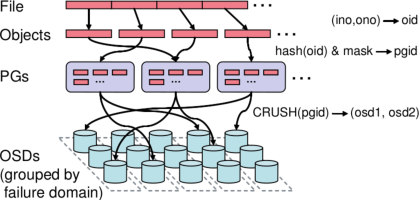
\includegraphics{crush.pdf}
\end{center}
\end{frame}

\section{Ceph - Praxis}
\subsection*{}

\begin{frame}
	\begin{center}
	\Large{Ceph Praxis}
	\end{center}
\end{frame}


\begin{frame}{Vorraussetzungen}
	\begin{itemize}
		\item Ausgeschaltetes Write Caching auf der Festplatte
		\item Dateisystem mit \emph{Extended Attributes (XATTRs)}:
		\begin{itemize}
			\item XFS
			\item BTRFS
%			\item Internet Status der Objekte
%			\item Snapshot Metadaten
%			\item RADOS Gateway Access Control Lists (ACLs).
		\end{itemize}
		\item Empfohlen: Disk f\"ur je OS/Ceph

	\end{itemize}
\end{frame}



\begin{frame}{Installation}

	Einfach, Pakete vorhanden f\"ur:
	\begin{itemize}
		\item Ubuntu
		\begin{itemize}
			\item natty
			\item oneiric
			\item precise
		\end{itemize}
		\item Debian
		\begin{itemize}
			\item sid
			\item squeeze
			\item wheezy
		\end{itemize}
		\item RPM 
		\begin{itemize}
			\item Selbst bauen per \texttt{rpmbuild}
		\end{itemize}
	\end{itemize}

\end{frame}


\begin{frame}{Cluster Design}
	3 Daemons
	\begin{itemize}
		\item ceph-osd: Object Storage
		\item ceph-mds: Metadaten Server: Verteilter, koh\"arenter Cache f\"ur Metadaten %agiert
		\item ceph-mon: Monitor, Cluster Management, Konfiguration und Zugangspunkt f\"ur CephFS
	\end{itemize}
\end{frame}


\begin{frame}{Object Storage Daemon}
	\begin{itemize}
		\item Mehrere OSDs pro Host m\"oglich
		\item Hardware:
		\begin{itemize}
			\item Viele Festplatten 
			\item Viel Ram (besseres Caching) (min. 500MB/Daemon)
			\item Schnelles Netzwerk
		\end{itemize}
		\item Anzahl:
		\begin{itemize}
			\item Mindestens 2, so viele wie m\"oglich
		\end{itemize}
	\end{itemize}
\end{frame}


\begin{frame}{Metadaten Daemon}
	\begin{itemize}

		\item Hardware:
		\begin{itemize}
			\item Sehr viel Ram
			\item Schnelle CPU
			\item Schnelles Netzwerk (geringe Verz\"ogerung)
		\end{itemize}
		\item Anzahl: 
		\begin{itemize}
			\item Mindestens 1
			\item 2 oder mehr f\"ur Redundanz und Load Balancing
		\end{itemize}
	\end{itemize}
\end{frame}


\begin{frame}{Monitor Daemon}
	\begin{itemize}
		\item Hardware:
		\begin{itemize}
			\item Einige GB Festplattenspeicher
			\item Feste IP
		\end{itemize}
		\item Anzahl:
		\begin{itemize}
			\item Ungerade Anzahl!
			\item 1 ist ok
			\item 3 ideal f\"ur die meisten Anwendungsf\"alle
			\item Mehr nur f\"ur sehr große Cluster
		\end{itemize}
	\end{itemize}
\end{frame}

\begin{frame}[fragile]{Beispiel ceph.conf}

\begin{lstlisting}
;This is a comment
[global]
	auth supported = cephx
[osd]
	osd journal size = 1000
[mon.a]
	host = myserver01
	mon addr = 10.0.0.101:6789
[mon.b]
	host = myserver02
	mon addr = 10.0.0.102:6789
[mon.c]
	host = myserver03
	mon addr = 10.0.0.103:6789
[osd.0]
	host = myserver01
[osd.1]
	host = myserver02
[osd.2]
	host = myserver03
[mds.a]
	host = myserver01
\end{lstlisting}
\end{frame}



\begin{frame}{Deployment}
	\begin{itemize}
		\item Chef cloud management tool (nicht getestet)
		\item \textbf{mkcephfs} (f\"ur Testzwecke)
			\begin{enumerate}
				\item Ben\"otigt passwortlosen \texttt{root}-Login auf allen Hosts
				\item Kopieren der ceph.conf auf alle Hosts
				\item Erstellen der Standardordner z.B. f\"ur myserver03
				\begin{description}
					\item \texttt{mkdir /var/lib/ceph/osd/ceph-2}
					\item \texttt{mkdir /var/lib/ceph/mon/ceph-c}
				\end{description}
				\item \texttt{mkcephfs -a -c /etc/ceph/ceph.conf -k /etc/ceph/ceph.keyring}
			\end{enumerate}
	\end{itemize}
\end{frame}



\begin{frame}{Zugriff}
	\begin{itemize}
		\item Kerneltreiber
		\item FUSE
		\item librados
		\item Rados Gateway (RESTful interface)
	\end{itemize}
\end{frame}

\begin{frame}{Probleme (CephFS)}
    \begin{itemize}
        \item Crash bei mount mit dem Kernel Treiber auf OSD-Server.
        \item Performance beim Kopieren von vielen Dateien noch gering.
    \end{itemize}
    \alert{Jedoch:} Selbstheilung sehr gut.
    %nur bei extremen Ausfaellen und Netz-beintraechtigung ging der Cluster in die Knie (degraded).
    %Nur einmal bei so einem Test gab es permanenten Datenverlust und wir mussten den cluster neu formatieren.
\end{frame}


\begin{frame}{Zusammenfassung}
\begin{itemize}
	\item Sehr vielversprechend
	\item Einiges unvollst\"andig implementiert 
	\item $\Rightarrow$ Warten auf stable
\end{itemize}
\end{frame}

\section{Fragen}
\subsection*{}
\begin{frame}
	\begin{center}
	\large Fragen? Anregungen? Vorschl\"age? Rants?
	\end{center}
	
	\begin{center}
	
\includegraphics[scale=0.8]{questions.jpg}
	\end{center}
\end{frame}



\begin{frame}{Literatur}
	\bibliographystyle{apalike}
	\bibliography{literature}	
\end{frame}

\end{document}


